\section{The butterfly factorisation for oscillatory integral operators}
\label{sec:butterfly}

Discrete Fourier integral operators (FIOs) have dense, oscillatory matrices, so a direct matrix--vector product is expensive. The butterfly algorithm obtains a faster representation by using low-rank approximations on specially chosen blocks. For the FIOs considered by Cand\`{e}s, Demanet, and Ying, these blocks and their accuracy can be understood through a centred expansion of the phase.\footnote{E.~J.~Cand\`{e}s, L.~Demanet, and L.~Ying, \emph{A Fast Butterfly Algorithm for the Computation of Fourier Integral Operators}, arXiv:0809.0719 (2008), especially Sections~1.1, 3, and~4; published in \emph{Multiscale Model. Simul.}~\textbf{7} (2009), 1727--1750.}

We first explain the mechanism in one dimension. Consider the oscillatory kernel
\begin{equation}
    K_n(x,p)=e^{2\pi i n\Psi(x,p)},
    \label{eq:scaled-kernel}
\end{equation}
where $\Psi$ is real and smooth. The parameter $n$ measures the frequency scale; it will also determine the depth of the block partition. The one-dimensional notation is simpler than that of the paper, but the essential estimate is unchanged.

\subsection{The centred rectangle expansion}

Let $A$ and $B$ be intervals of widths $h_A$ and $h_B$, centred at $a$ and $b$. On the rectangle $A\times B$, define the double difference
\begin{equation}
    R_{AB}(x,p)
    =\Psi(x,p)-\Psi(a,p)-\Psi(x,b)+\Psi(a,b).
    \label{eq:rectangle-remainder}
\end{equation}
This gives the exact factorisation
\begin{equation}
    K_n(x,p)
    =e^{2\pi i n\Psi(x,b)}
     e^{2\pi i n\Psi(a,p)}
     e^{-2\pi i n\Psi(a,b)}
     e^{2\pi i nR_{AB}(x,p)}.
    \label{eq:centered-factorisation}
\end{equation}
The first three factors are respectively a function of $x$, a function of $p$, and a constant. They do not prevent a separated approximation. The fourth factor contains the part that still couples $x$ and $p$.

After sampling $x_i\in A$ and $p_j\in B$, the same identity can be written
\begin{equation}
    K_{AB}=c_{AB}D_AH_{AB}D_B,
    \qquad (H_{AB})_{ij}=e^{2\pi i nR_{AB}(x_i,p_j)},
\end{equation}
where $c_{AB}=e^{-2\pi i n\Psi(a,b)}$ and $D_A,D_B$ are unit-modulus diagonal matrices containing the other two factors. Multiplication by these diagonal matrices preserves every singular value. It is therefore enough to study the compressibility of $H_{AB}$. This is also why block compression does not contradict global rank: for the $N\times N$ Fourier matrix, $K/\sqrt{N}$ is unitary, so every singular value of $K$ equals $\sqrt{N}$. The full Fourier matrix has full rank; useful compression appears only in appropriate subblocks.

The fundamental theorem of calculus gives
\begin{equation}
    R_{AB}(x,p)
    =\int_a^x\int_b^p \partial_s\partial_t\Psi(s,t)
      \,\mathrm{d}t\,\mathrm{d}s.
    \label{eq:mixed-integral}
\end{equation}
Consequently, if
$M_{AB}=\sup_{A\times B}|\partial_x\partial_p\Psi|$, then
\begin{equation}
    |R_{AB}(x,p)|
    \leq M_{AB}|x-a|\,|p-b|
    \leq \frac{M_{AB}h_Ah_B}{4}.
    \label{eq:rectangle-bound}
\end{equation}
Thus the residual phase satisfies
\begin{equation}
    2\pi n|R_{AB}(x,p)|
    \leq \rho_{AB},
    \qquad
    \rho_{AB}:=\frac{\pi}{2}M_{AB}n h_Ah_B.
    \label{eq:residual-phase-bound}
\end{equation}
The important quantity is the product $n h_Ah_B$, not $h_A$ or $h_B$ separately, and not the total size of the original phase. Large terms involving $\Psi_x$ or $\Psi_p$ have been removed exactly in~\eqref{eq:centered-factorisation}.

For square boxes in two dimensions, the analogous estimate follows by applying the same argument coordinate by coordinate and summing the mixed partial derivatives. This is precisely the $O(1/n)$ estimate for $R_{AB}$ used by Cand\`{e}s--Demanet--Ying when $h_Ah_B\leq 1/n$.

\subsection{Why the remainder gives a low-rank block}

A separated approximation
\begin{equation}
    K_n(x,p)\approx \sum_{r=1}^{q}\alpha_r(x)\beta_r(p),
    \qquad x\in A,\quad p\in B,
    \label{eq:separated-block}
\end{equation}
is a rank-at-most-$q$ approximation after discretisation.

The error norm must be stated explicitly. The estimates below are uniform kernel bounds, meaning $|E_{ij}|\leq\varepsilon$ on the sampled entries. For an $m_A\times m_B$ block, they imply
\begin{equation}
    \|E\|_2\leq\|E\|_F\leq\varepsilon\sqrt{m_Am_B}.
\end{equation}
They do not by themselves give numerical rank at absolute spectral tolerance $\varepsilon$; that requires $\|E\|_2\leq\varepsilon$, while a relative spectral tolerance uses $\|E\|_2\leq\varepsilon\|K_{AB}\|_2$. The numerical figures below instead show relative Euclidean error in the computed output vectors, as stated in their captions.

The bilinear example makes the connection with~\eqref{eq:residual-phase-bound} explicit. Suppose $\Psi(x,p)=xp$. Then
\begin{equation}
    R_{AB}(x,p)=(x-a)(p-b),
    \qquad
    |2\pi nR_{AB}|\leq\rho_{AB}.
\end{equation}
Taylor expansion of the exponential gives
\begin{equation}
    e^{2\pi i nR_{AB}}
    =\sum_{r=0}^{q-1}
     \frac{(2\pi i n)^r}{r!}(x-a)^r(p-b)^r
     +\mathcal{E}_q(x,p),
    \qquad
    |\mathcal{E}_q|\leq\frac{\rho_{AB}^q}{q!}.
    \label{eq:bilinear-exponential}
\end{equation}
Every term in the sum is a product of a function of $x$ and a function of $p$. Multiplication by the three unit-modulus factors in~\eqref{eq:centered-factorisation} preserves both the separation rank and the error bound. Hence the original oscillatory block has a rank-$q$ approximation whose error is at most $\rho_{AB}^q/q!$. If $\rho_{AB}$ is held at a fixed value independent of $n$, the order required for a prescribed local tolerance is also independent of $n$.

For a general phase, $R_{AB}$ is not a product $(x-a)(p-b)$, and the factorial estimate in~\eqref{eq:bilinear-exponential} need not hold. Cand\`{e}s--Demanet--Ying instead assume that $\Psi$ is real-analytic in the joint variables. They use truncated Taylor sums to prove low rank and construct the approximation by tensor-product Chebyshev interpolation of $e^{2\pi i nR_{AB}}$. One interpolates in $p$ when $B$ is the smaller box and in $x$ when $A$ is the smaller box. After restoring the factors in~\eqref{eq:centered-factorisation}, the procedure is: \emph{prefactor the oscillation, interpolate the residual, and remodulate}.

Equation~\eqref{eq:rectangle-bound} alone is not a low-rank proof: higher mixed derivatives also enter the Taylor or interpolation error. In their two-dimensional setting, Theorem~3.1 concerns square boxes with $h_Ah_B=1/n$ and real-analytic phases. It gives constants $N_0$ and $\varepsilon_0$ such that, for $n\geq N_0$ and $\varepsilon\leq\varepsilon_0$, the block has an $\varepsilon$-accurate separated approximation of rank $r_\varepsilon=O(\log^4(1/\varepsilon))$. The implied constant is independent of $n$. This is a statement about each complementary block, not about the rank of the full matrix.

\subsection{Complementary boxes keep the local error uniform}
\label{subsec:complementary-boxes}

The block partition is built from two dyadic trees, one for observation points and one for source points. Take both domains to be $[0,1]$ in the one-dimensional model. Assume that $n$ is a power of two and let each tree have depth $L=\log_2 n$. A box at level $\ell$ has width $2^{-\ell}$.

At step $\ell$, choose an observation box $A_\ell$ at tree level $\ell$, but a source box $B_{L-\ell}$ at the complementary level $L-\ell$. Their widths are
\begin{equation}
    h_\ell=2^{-\ell},
    \qquad
    H_\ell=2^{-(L-\ell)}=\frac{2^\ell}{n},
    \qquad
    h_\ell H_\ell=2^{-L}=\frac1n.
    \label{eq:ladder-widths}
\end{equation}
As $\ell$ increases, observation boxes split and become narrower, while source boxes merge in pairs and become wider. At the beginning, $A$ is the root and $B$ is a leaf; at the end, $A$ is a leaf and $B$ is the root.

If $M$ is a uniform bound for $|\partial_x\partial_p\Psi|$, then~\eqref{eq:residual-phase-bound} and~\eqref{eq:ladder-widths} give
\begin{equation}
    \rho_\ell
    \leq \frac{\pi}{2}M n h_\ell H_\ell
    =\frac{\pi}{2}M
    \qquad\text{at every level}.
    \label{eq:constant-residual}
\end{equation}
The opposite traversal of the two trees therefore preserves the width product and the residual-phase bound. It also gives exactly $n$ complementary pairs at each level.

In the bilinear example,~\eqref{eq:constant-residual} implies that the same $q$ in~\eqref{eq:bilinear-exponential} gives the same local error bound at every level. In the analytic theorem, the hypotheses hold on every complementary pair, so its rank bound is also uniform over the ladder. Near the middle level, both widths are approximately $n^{-1/2}$. This is where the algorithm changes from interpolation in the source variable to interpolation in the observation variable, always choosing the smaller box.

The word \emph{local} matters. A uniform error on every block does not, by itself, bound the error of the complete multilevel recursion; propagated errors must also be tracked. The geometric estimate explains why no level intrinsically requires a larger rank than another.

\subsection{From low-rank blocks to the butterfly recursion}
\label{subsec:butterfly-recursion}

For any source box $B$, define the partial potential
\begin{equation}
    u_B(x)=\sum_{p_j\in B}K_n(x,p_j)f(p_j).
\end{equation}
A rank-$r$ approximation on $A\times B$,
$K_n(x,p)\approx\sum_{t=1}^{r}\alpha_t^{AB}(x)\beta_t^{AB}(p)$, reduces this potential on $A$ to
\begin{equation}
    u_B(x)\approx\sum_{t=1}^{r}\alpha_t^{AB}(x)\delta_t^{AB},
    \qquad
    \delta_t^{AB}=\sum_{p_j\in B}\beta_t^{AB}(p_j)f(p_j).
    \label{eq:compressed-potential}
\end{equation}
Only $r$ coefficients are needed to describe the contribution of $B$ throughout $A$.

The butterfly algorithm avoids calculating these coefficients independently from all the sources in every large box. At the next level, $A$ is replaced by one of its children and $B$ by its parent. The approximations already available on the parent of $A$ and the children of $B$ are recombined, after which the new complementary low-rank representation compresses them again. Thus short coefficient vectors are transferred through the levels by small matrices. At the last level, $B$ is the whole source domain and~\eqref{eq:compressed-potential} is evaluated on each observation leaf.

At a fixed level of the one-dimensional ladder, there are $2^\ell$ observation boxes and $2^{L-\ell}$ source boxes, hence $2^L=n$ complementary pairs. Across the $L+1$ levels this gives $O(n\log n)$ pairs. If the rank is fixed, the work per pair is also fixed, so the recursive updates cost $O(n\log n)$. In the paper's two-dimensional quadtree construction, the same count gives $N^2$ pairs per level and $O(N^2\log N)$ pairs in total. For a fixed tolerance, this yields the paper's $O(N^2\log N)$ operation count.

These counts concern the explicit-kernel butterfly traversal and application, not the separate task of constructing a general butterfly factorisation from a matrix alone. For the matrix-side construction of Li et al., applying the resulting sparse factors costs $O(N\log N)$. Their construction costs $O(N^{3/2})$ when blocks are sampled directly, or $O(C_K(N)\sqrt N+N^{3/2})$ using black-box applications of the matrix and its adjoint, where $C_K(N)$ is one such application. When $C_K(N)=O(N\log N)$, the latter becomes $O(N^{3/2}\log N)$. These are different algorithms and should not be conflated.

\subsection{The complementary low-rank condition}
\label{subsec:complementary-low-rank}

The same structure can be described entirely in matrix language. Let $K$ be a matrix whose row and column indices are organised by trees $T_X$ and $T_P$ of depth $L$. It satisfies the \emph{complementary low-rank property} if, for a prescribed absolute spectral tolerance $\varepsilon$, every block
\begin{equation}
    K_{A,B},\qquad A\in T_X,\quad B\in T_P,
    \quad \ell(A)+\ell(B)=L,
\end{equation}
can be approximated to this accuracy in spectral norm with rank at most $r_\varepsilon$, where $r_\varepsilon$ is small compared with the matrix dimensions. General butterfly factorisations assume this property and convert the collection of block approximations into a product of sparse factors.\footnote{Y.~Li, H.~Yang, E.~R.~Martin, K.~L.~Ho, and L.~Ying, \emph{Butterfly Factorization}, \emph{Multiscale Model. Simul.}~\textbf{13} (2015), 714--732; arXiv:1502.01379.}

For uniformly refined square boxes, $\ell(A)+\ell(B)=L$ means that $h_Ah_B$ is of order $2^{-L}$. In the FIO normalisation above, this is exactly $1/n$. The centred expansion therefore supplies an analytic explanation for the complementary low-rank assumption: the double difference contains only mixed derivatives, and the width-product condition bounds the residual phase uniformly. For the analytic FIOs considered here, the theorem quoted above verifies the required rank bound.

This is not the usual statement that only well-separated, off-diagonal blocks are low rank. Complementary pairs cover the whole matrix, including geometrically close boxes; the saving comes from replacing every such block by a short separated expansion, not from discarding interactions. Nor is the property automatic for every oscillatory or Green-function matrix. Smoothness of the transformed phase and the validity of the width-product estimate are essential.

Finally, we relate the notation to the original paper. Cand\`{e}s--Demanet--Ying consider two-dimensional operators with a phase $\Phi(x,k)$ homogeneous of degree one in $k$. The polar rescaling $k=(N/\sqrt2)\,p_1v(p_2)$, where $v(p_2)=(\cos 2\pi p_2,\sin 2\pi p_2)$, gives $\Phi(x,k)=N\Psi(x,p)$ with $\Psi(x,p)=\Phi(x,v(p_2))p_1/\sqrt2$. Thus the kernel becomes $e^{2\pi i N\Psi(x,p)}$ with $x,p\in[0,1]^2$. Their square boxes satisfy $w(A)w(B)=1/N$, which is the two-dimensional counterpart of~\eqref{eq:ladder-widths}. Thus the one-dimensional calculation above isolates the central idea without changing its geometric content.

\subsection{A numerical check using the discrete Fourier transform}
\label{subsec:butterfly-dft-demo}

The bilinear case gives a direct numerical check. Take $N$ observation and source points $x_i=i/N$ and $p_j=j/N$, where $i,j=0,\ldots,N-1$. Then
\begin{equation}
    e^{2\pi i N\Psi(x_i,p_j)}
    =e^{2\pi i ij/N},
\end{equation}
so $\Psi(x,p)=xp$ gives the positive-sign discrete Fourier transform. NumPy's default inverse FFT includes the normalisation $1/N$:
\begin{equation}
    \operatorname{IFFT}(f)_i
    =\frac1N\sum_{j=0}^{N-1}e^{2\pi i ij/N}f_j.
\end{equation}
Consequently $u=N\,\operatorname{IFFT}(f)$ is the desired positive-sign transform, computed exactly up to floating-point roundoff.

Figure~\ref{fig:butterfly-dft-demo} compares this reference with the centred-residual algorithm. The implementation is provided in the folder \texttt{butterfly-demo}. The Taylor calculation above is an error model; the implementation instead uses Chebyshev interpolation of the residual exponential, as described earlier. Increasing $q$ rapidly decreases the approximation error. The top-right panel explicitly plots this error against $N$: at fixed $q=8$ it remains approximately constant over the tested sizes. The implementation performs $N$ complementary paired updates at each level, and the timing panel includes both an $N\log N$ guide and an $N^2$ guide. Wall time is not the main comparison: the FFT is an optimised algorithm specialised to this transform, whereas the Python butterfly code is a minimal demonstration. These numerical checks are empirical; they are not a proof of a global error bound.

\begin{figure}[htbp]
    \centering
    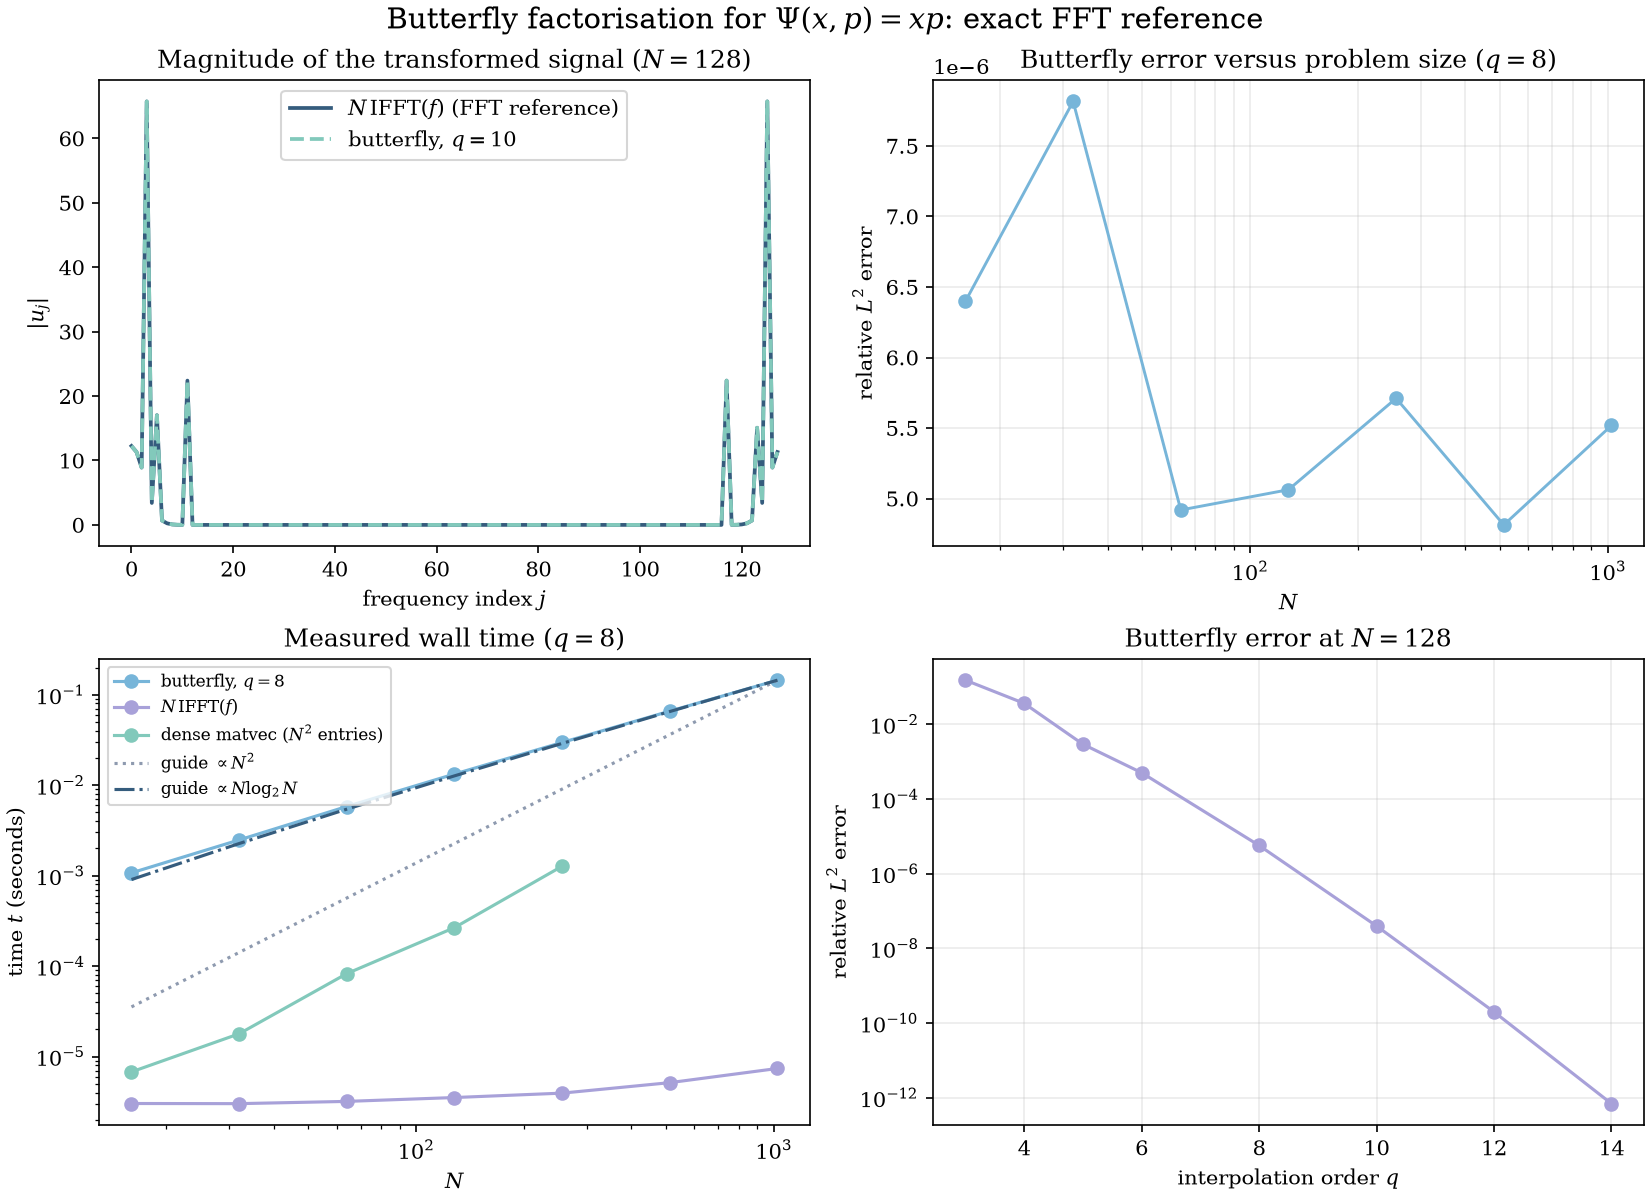
\includegraphics[width=\textwidth]{butterfly-demo/results/comparison.png}
    \caption{Comparison of the butterfly algorithm with the exact FFT reference for $\Psi(x,p)=xp$. \emph{Top left:} transformed magnitudes for a complex test signal at $N=128$, using $q=10$; the two curves are nearly indistinguishable. \emph{Top right:} relative Euclidean output error versus $N$ at fixed $q=8$, shown separately from the dependence on $q$. \emph{Bottom left:} single-thread wall times at $q=8$ for $N=16,\ldots,1024$, including a dense matrix--vector product for $N\leq256$ and guides proportional to $N\log_2N$ and $N^2$. The dense path was warmed up before timing; absolute times are machine dependent. \emph{Bottom right:} relative $L^2$ error $\|u_q-u_{\mathrm{FFT}}\|_2/\|u_{\mathrm{FFT}}\|_2$ at $N=128$ as the Chebyshev interpolation order $q$ varies. All approximation errors use $u_{\mathrm{FFT}}=N\,\operatorname{IFFT}(f)$ as the reference.}
    \label{fig:butterfly-dft-demo}
\end{figure}

\subsection{A non-DFT oscillatory example}
\label{subsec:non-dft-demo}

To check that the construction is not tied to the Fourier transform, consider
\begin{equation}
    \Psi(x,p)=xp+0.1x^2p^2.
    \label{eq:non-dft-phase}
\end{equation}
This is still real-analytic, but $R_{AB}$ is no longer simply $(x-a)(p-b)$. The explicit Taylor estimate for the bilinear example therefore does not apply; the local approximation is constructed by residual interpolation.

Figure~\ref{fig:non-dft-demo} uses this phase in the same implementation, now comparing against an explicit dense evaluation of
$Kf$, not against an FFT. The transformed magnitudes at $q=10$ agree closely, and increasing $q$ again rapidly reduces the relative Euclidean output error. This is an additional numerical test of the approximation, not a claim of a global diagonalisation or a global error estimate.

\begin{figure}[htbp]
    \centering
    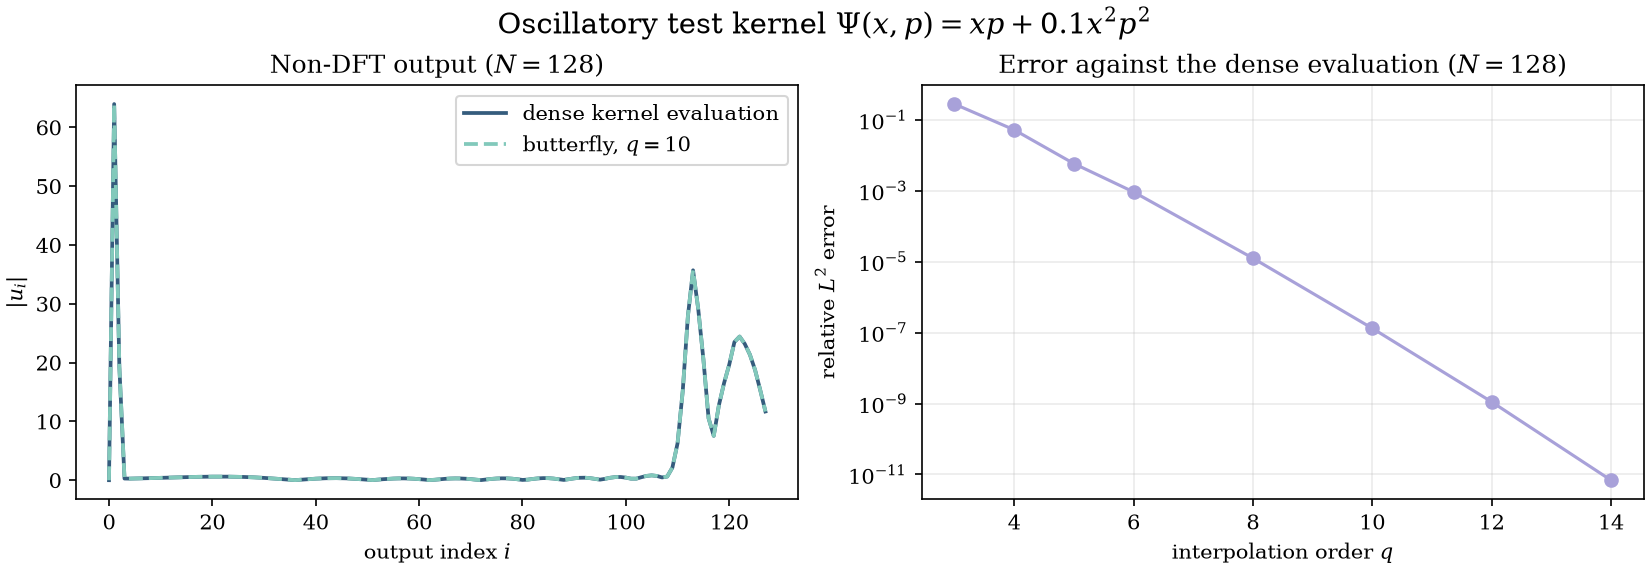
\includegraphics[width=\textwidth]{butterfly-demo/results/non_dft_comparison.png}
    \caption{Application to the non-DFT oscillatory test kernel $\Psi(x,p)=xp+0.1x^2p^2$ at $N=128$. \emph{Left:} output magnitudes from the explicit dense kernel evaluation and from the butterfly algorithm at $q=10$. \emph{Right:} relative $L^2$ error $\|u_q-u_{\mathrm{dense}}\|_2/\|u_{\mathrm{dense}}\|_2$ against the Chebyshev interpolation order $q$. Unlike the DFT comparison, the reference here is computed entirely by dense evaluation of~\eqref{eq:non-dft-phase}.}
    \label{fig:non-dft-demo}
\end{figure}
